

\section{Friday}\index{week4_Friday_lecture}

This lecture will finish the topic for continuity, and we will have a very simple, easy quiz on Sunday.

\subsection{Continuity Analysis}
\begin{definition}[Lipschitz Continuity]
A function $f$ is \emph{Lipschitz continuous} at $x_0$ if there exists a constant $M$ (depend on $x_0$) such that
\[
|f(x) - f(x_0)|\le M|x - x_0|,
\]
for $\forall|x-x_0|$ small.
\end{definition}
\begin{remark}
\begin{itemize}
\item
Note that Lipschitzness places a upper bound on the growth of the funciton that is linear in the perturbation, i.e., $|x-x_0|$. 
\item
Also notice that Lipschitz functions need not be differentiable, e.g., $f(x) = |x|$ is Lipschitz continuous at $x=0$.
\item
However, differentiable functions with bounded derivative are always Lipschitz.
\item
Lipschitz continuous functions are always continuous. (choose $\delta =\varepsilon/M$)
\end{itemize}
\end{remark}
A property similar to Lipschitzness is that of Holder continuity.
\begin{definition}[Holder]
A function $f$ is said to be \emph{Holder continuous} of order $\alpha$ at $x_0$ if there exists a constant $M$ such that 
\[
|f(x) - f(x_0)|\le M|x-x_0|^\alpha
\]
for $\forall |x-x_0|$ small, where $0<\alpha<1$.
\end{definition}
\begin{remark}
\begin{itemize}
\item
$f(x) = \sqrt{|x|}$ is Holder continuous of order $1/2$ at $x=0$.
\item
Holder continuous functions are always continuous (choose $\delta =(\varepsilon/M)^{1/\alpha}$)
\end{itemize}
\end{remark}
\paragraph{Holder Continuity for Differentiable Equation}
Solving differentiable equations is a core topic in pure math. When solving the ODE $u''=f(x)$ with $f$ continuous, we can say $u\in\mathcal{C}^{2}$. However, when talking about the PDE $u_{xx}+u_{yy} = f(x,y)$ with continuous $f$, $u$ is not necessarily twice continuously differentiable. Instead, $u$ is almost $\mathcal{C}^2$. However, if given the extra condition $f\in\mathcal{C}_{\text{holder}}^\alpha$, then we imply $u\in\mathcal{C}^{2+\alpha}$. Holder continuous is vital important for future mathematics study.
\begin{definition}[Convex]
A funciton $f$ is said to be \emph{convex} in $(a,b)$ if 
\[
f(tx + (1-t)y) \le tf(x) + (1-t) f(y)
\]
holds for $\forall x,y\in(a,b)$ and $\forall t\in[0,1]$
\end{definition}
\begin{remark}
The geometrically meaning for convexity is that the function evaluated in the line segment is lower than secant line between $x$ and $y$, i.e., a convex function $f$ lies below secant line.
\begin{figure}[H]
\centering
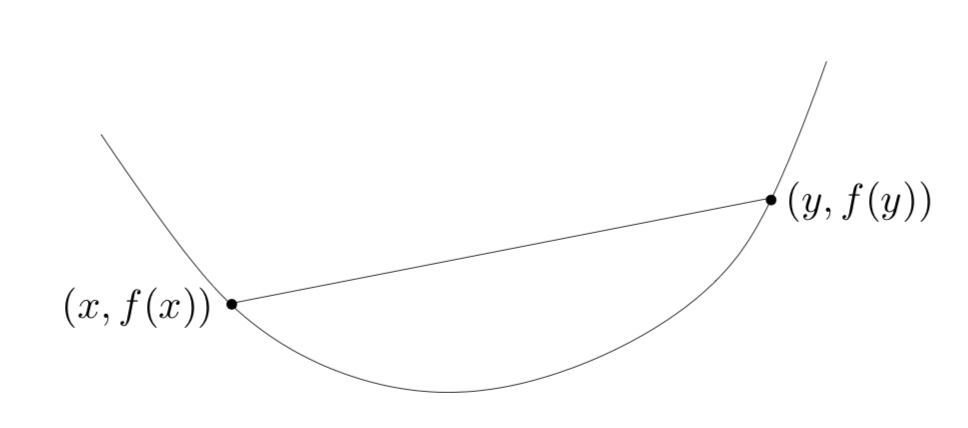
\includegraphics[width=8cm]{week4/4_4.png}
\caption{Graph of a convex function. The line segment between any two points on the graph lies above the graph.}
\end{figure}
\end{remark}
\begin{figure} 
  \subfigure[Pick $x$ and $y$ at either side of $z$]{ 
    \label{fig:mini:subfig:a} %% label for first subfigure 
    \begin{minipage}[b]{0.5\textwidth} 
      \centering 
      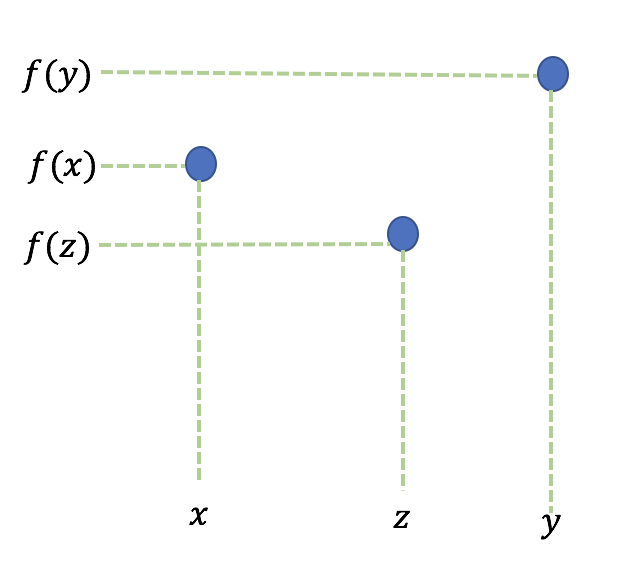
\includegraphics[width=2.5in]{week4/4_5.png} 
    \end{minipage}}% 
  \subfigure[The point $y$ is above the secant line]{ 
    \label{fig:mini:subfig:b} %% label for second subfigure 
    \begin{minipage}[b]{0.5\textwidth} 
      \centering 
      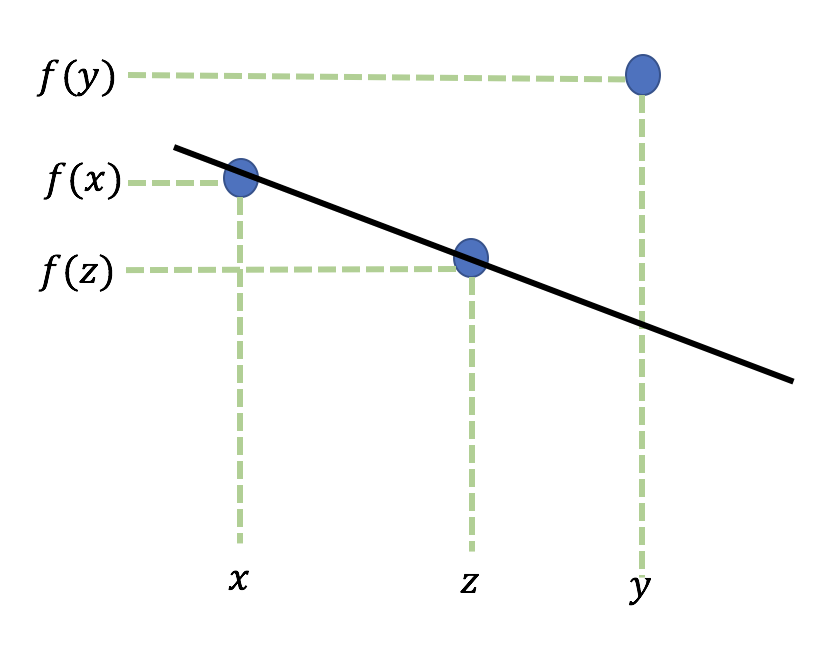
\includegraphics[width=2.5in]{week4/4_6.png} 
    \end{minipage}} 
    \subfigure[The point $x$ is below the secant line]{ 
    \label{fig:mini:subfig:a} %% label for first subfigure 
    \begin{minipage}[b]{0.5\textwidth} 
      \centering 
      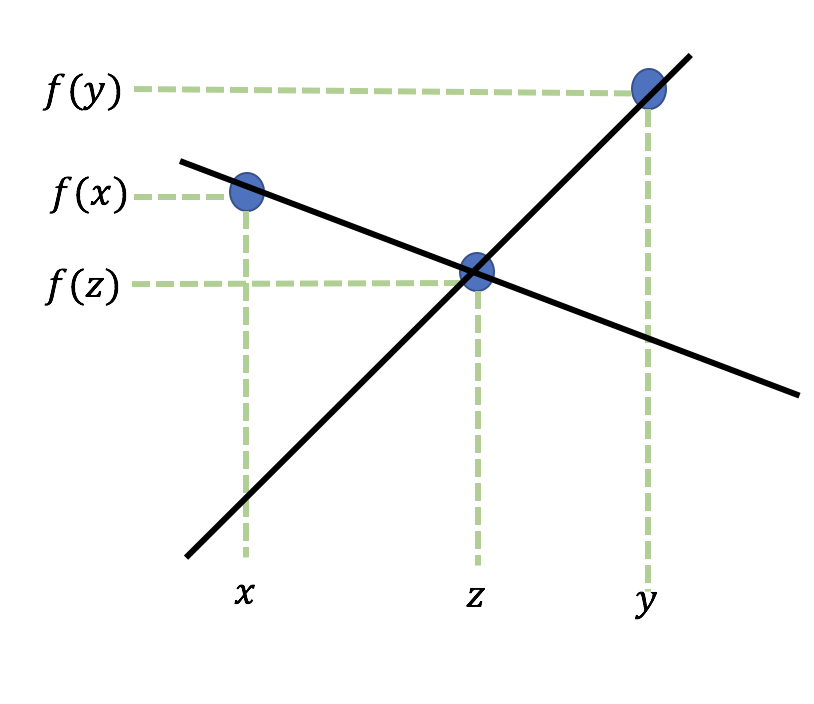
\includegraphics[width=2.5in]{week4/4_7.png} 
    \end{minipage}}% 
  \subfigure[The function is inside the red region]{ 
    \label{4:4:d} %% label for second subfigure 
    \begin{minipage}[b]{0.5\textwidth}
      \centering 
      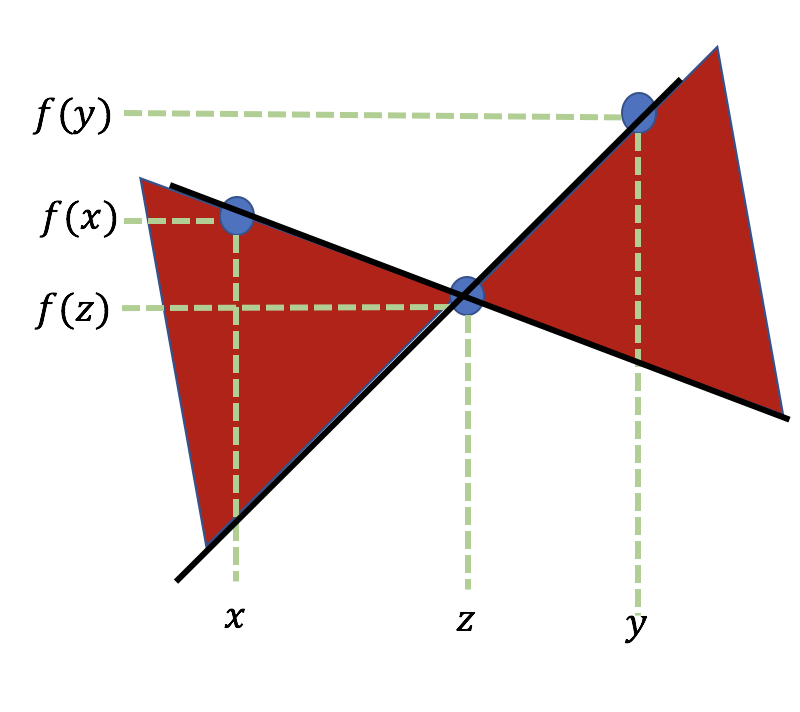
\includegraphics[width=2.5in]{week4/4_8.png} 
    \end{minipage}} 
  \caption{Graphic Proof for Proposition(\ref{Pro:4:5})} 
  \label{Graphic_proof} %% label for entire figure 
\end{figure}

An intuitive statement is that a convex function is always continuous. This statement can be shown pictorially.
\begin{proposition}\label{Pro:4:5}
A convex function must be continuous.
\end{proposition}
\begin{proof}
The proof is given in Fig:(\ref{Graphic_proof}):
\begin{itemize}
\item
To show the continuity for $z$, pick $x$ and $y$ at either side.
\item
By convexity, the $y$ lies above the secant line between $x$ and $z$, otherwise draw a secant line between $x$ and $y$, then $z$ lines above the secant line (contradiction).
\item
Again, $x$ lines below the secant line between $z$ and $y$.
\item
Hence, the function lies inside the red region shown in Fig:(\ref{4:4:d}).
\item
Pick a sequence $\{z_n\}\to z$, the function $f(z_n)$ must converge to $f(z)$.
\end{itemize}
The proof is complete.
\end{proof}
The following two statements are left as exercise:
\begin{proposition}
Assume that $f$ is continuous real function defined in $(a,b)$ such that
\[
f\left(\frac{x+y}{2}\right)\le\frac{f(x) + f(y)}{2}
\]
for all $x,y\in(a,b)$. Then $f$ is convex.
\end{proposition}
\begin{remark}
We can pick an example to show that dropping out the continuity condition will make this statement false.
\end{remark}


\subsection{Monotone Analysis}
\begin{definition}[Monotone]
The function $f$ is said to be \emph{monotone increasing} (\emph{decreasing}) if $f(x)\le f(y)$ ($f(x)\ge f(y)$) whenever $x<y$.
\end{definition}
\begin{remark}
\begin{itemize}
\item
For monotone functions,
\[
\begin{array}{ll}
\lim_{x\to x_0+}f(x),
&
\lim_{x\to x_0-}f(x),
\end{array}
\]
always exist.
\item
The difference 
\[
\lim_{x\to x_0+}f(x)-\lim_{x\to x_0-}f(x)
\]
is called the \emph{jump discontinuity} at $x=x_0$.
\end{itemize}
\end{remark}
\begin{proposition}
A monotone function $f$ on $(a,b)$ is continuous except at possibly a countable number of points.
\end{proposition}
We show the statement is true for interval $[a+\frac{1}{n},b-\frac{1}{n}]$ first. That's because the function inside a closed intercal is finite.
\begin{proof}
\begin{itemize}
\item
Let $S_k$ denote the set of all points in $[a+\frac{1}{n},b-\frac{1}{n}]$ on which $f$ has a jump discontinuity no less than $\frac{1}{k}$.
\item
Then the set $S_k$ must be finite for every $k$, otherwise the total jump of $S_k$ will be infinite, which contradicts the range of $f$.
\item
The set of all discontinuous points of $f$ on $[a+\frac{1}{n},b-\frac{1}{n}]$ is the union $\bigcup_{k=1}^\infty S_k$, therefore is at most countable.
\item
Note that 
\[
(a,b)=\bigcup_{n=1}^\infty[a+\frac{1}{n},b-\frac{1}{n}],
\]
the countably union of at most countable sets is at most countable. Tshe proof is complete.
\end{itemize}
\end{proof}
\paragraph{Exercise} Given the Riemann function 
\[
f(x)=\left\{
\begin{aligned}
0,&\quad x\in\mathbb{Q}\\
\frac{1}{q},&\quad x=\frac{p}{q}, (p,q)=1.
\end{aligned}
\right.
\]
Is $f$ Lipschitz continuous, Holder continuous, or whatever at the given point $x_0\notin\mathbb{Q}$?
\subsection{Cantor Set}
Now we describe a complicated subset of $\mathbb{R}$ which is uncountable. This set is called the Cantor set.
\paragraph{Geometric description}
We start with the unit interval
\[
F_0=[0,1]
\]
Now define a new set
\[
F_1 = F_0\setminus(\frac{1}{3},\frac{2}{3})=[0,1/3]\bigcup[2/3,1],
\]
i.e., we obtain $F_1$ by deleting the open middle third of $F_0$.

Next we obtain a new set $F_2$ by deleting the open middle thirds of each of the intervals making up $F_1$:
\[
F_2 = [0,1/9]\bigcup[2/9,1/3]\bigcup[2/3,7/9]\bigcup[8/9,1]
\]
Continue in this way to obtain sets $F_n$, $n\ge 0$, where $F_n$ consists of $2^n$ disjoint closed intervals of length $3^{-n}$, formed by deleting the middle thirds of the intervals making up $F_{n-1}$.

The \emph{Cantor set} is defined to be the intersection of these sets:
\[
F=\bigcup_{n=1}^\infty F_n
\]
\paragraph{Arithmetic description}
We also have
\[
F=\left\{
x\in[0,1]: x=\sum_{n=1}^\infty a_n3^{-n}, a_n\in\{0,2\},n\ge1
\right\}
\]
Here we can also describe $F$ as the set of reals with a tenary expansion
\[
0.a_1a_2\dots a_n\dots\qquad\qquad
a_n\in\{0,2\}.
\]
For example, given $x=3/4$, how to find the tenary expansion $x\sim0.a_1a_2\dots$? Clearly $3/4\in[\frac{2}{3},1]$, i.e., $a_1=1$. The next interval is determined by which interval among $[\frac{2}{3},\frac{7}{9}]$ and $[\frac{8}{9},1]$ that $x$ belongs. It is clearly that it belongs to the first interval, and so $a_2=0$. Thus we can find $a_n$ recursively via this way to get the tenary expansion.



\begin{proposition}
There is a one-to-one correspondence between $F$ and $F_0$.
\end{proposition}
\begin{proof}
For any $x\in F$, we write $x=0.a_1a_2\cdots a_j$ with $a_j=0$ or $2$. Also, we can construct our $y=0.b_1b_2\cdots$ with $b_j=\frac{a_j}{2}$, i.e., $y$ is any number with binary expansion. Therefore, we establishes a one to one correspondence between $F$ and the set of points in $(0,1).$
\end{proof}
Also, there is a one-to-one correspondence between $F$ and $F_0$ implies $F$ is \emph{uncountable}.
\begin{proposition}
The measure of $F$ is $0$.
\end{proposition}
\begin{proof}
The $F_1$ is constructed by taking away an interval with length $\frac{1}{3}$. The $F_2$ is constructed by taking away intervals with total length $\frac{2}{9}$, etc. Therefore, the toal length of taking-away intervals is given by:
\begin{align*}
\frac{1}{3}+\frac{2}{9}+\frac{4}{27}+&\cdots\\
&=\frac{1}{3}+\frac{2}{3^2}+\frac{4}{3^3}+\cdots\\
&=\frac{1}{3}(1+\frac{2}{3}+(\frac{2}{3})^2+\cdots)\\
&=1
\end{align*}
\end{proof}
\begin{proposition}
$F$ is closed and nowhere dense.
\end{proposition}
\begin{proof}
$F$ is closed since it is the complement of the union of open intervals. The Cantor set is nowhere dense as its closure has empty interior.
\end{proof}
The proof for proposition(\ref{Pro:4:11}) is left as exercise.
\begin{proposition}\label{Pro:4:11}
Every point in $F$ is a limit point of $F$
\end{proposition}
\begin{definition}[Perfect]
A closed set $\bm S$ is \emph{perfect} if every point in $\bm S$ is a limit point of $\bm S$.
\end{definition}
The proof for proposition(\ref{Pro:4:12}) is left as exercise.
\begin{proposition}\label{Pro:4:12}
Any perfect set is uncountable.
\end{proposition}















